\chapter{Introduction} % Main chapter title
%\selectlanguage{serbianc}
%\sffamily
%\fontencoding{OT2}\fontfamily{Tempora-TLF}\selectfont


Many real systems, such as brain networks, social organisations, cities or cells, consist of large number of interacting units and belong to a class commonly known as complex systems.
%Many real systems, such as brain networks, social organisations, cities or even biological systems, can be represented as complex systems. 
%The common property of these systems is that they are composed of many interacting elements. 
%%TODO Reprezentacija je kompleksna mreza, sistemi su kompleksni. To je njiihova inherentna osobina. Umesto ove recenice ja bih napisala sledece: "Many real systems, such as brain networks, social organisations, cities or cells, consist of large number of interacting units and belong to a class commonly known as complex systems." bez recenice the common property.
One of the most prominent characteristics of complex systems is that they exhibit emergent collective behavior that can not be predicted based on the behavior of individual components. The interactions between system components can be represented as a complex network \cite{kwapien2012}. The emergence of collective behavior strongly depends on the structure of network of interactions.
%Still, to describe the properties of the system, we can only conclude a little from the behaviour of a single individual. 
%%TODO "One of the most prominent characteristics of complex systems is that they exhibit emergent collective behavior that can not be predicted based on the behavior of individual components." I izbacila bih sledecu recenicu, jedino bih citat bih stavila u ovu recenicu. I posle toga bih dodala jos dve recenice:"The interactions between system components can be represented as a complex network \citat. The emergence of collective behavior strongly depends on the structure of network of interactions." I onda nastavis "The structure of the brain ..." do kraja paragrafa
%Due to specific interactions, without any central force, in the complex system, the collective behaviour \cite{kwapien2012} emerges. 
The structure of the brain network and its properties are fundamental for brain functioning, while an emergent phenomenon is human intelligence. In societies, people's interactions lead to civilisation, economy, formation of social groups. Also, the animal populations show different levels of organisation: such as patterns in bird flocks or schools of fish \cite{thurner2018}.

The interactions between the complex system elements are not homogeneous; as systems evolve, they can also change \cite{thurner2018}. The research in complex systems mainly focuses on the interactions between its units. Knowing the shape of these connections, we can determine the properties of the system \cite{ladyman2013}. We can construct a representation with neurons and synapses representing connectivity in the brain network. Neurons in the same brain area are closely connected \cite{latora2017complex}.
Similarly, we can define communication between people. The structure of these interactions gives us insights, for example, how information propagates through the system. The presence of people with many connections can lead to faster information flow. 

The universality is an important property of the complex systems  \cite{binney1992}. For example, the time lap between two email messages follows the power-law distribution \cite{garas2012emotional}, and the exponent is universal across different platforms. Similar conclusions are found in distributions of the votes in elections \cite{fortunato2007scaling, chatterjee2013}, and citations of scientific publications \cite{radicchi2008}. Even the growth of social groups, such as cities, follows universal patterns. The probability distribution of the city sizes in one country follows the same laws, with a similar exponent for all countries \cite{barthelemy2019, fazio2015pareto}. However, the distribution of company sizes follows log-normal behaviour and remains stable over decades \cite{amaral1997scaling, stanley1996scaling}. Understanding how universality emerges in different systems is the focus of the statistical physics of the complex systems \cite{verbavatz2020}. 

%TODO motivacioni paragraf

Despite the differences between complex systems, they can be studied using the same techniques. The natural extension of the complex system is the network, sets of nodes (vertices) and links (edges). Elements in the system are nodes, while interactions between them are given as edges. This approximation allows us to treat equally social \cite{myers2014, sarigol2014} (graph of actors), biological (network of proteins) \cite{fraiman2009ising, schneider2011modeling} or even technological systems (internet, traffic) \cite{costa2007characterization, costa2011analyzing, newman2003structure}. 

The complex network theory originates from the graph theory in mathematics. The first problem solved using graph theory was the $Konigsberg$ problem of seven bridges. The city of $Konigsberg$ had seven bridges connecting the city's parts across the river and the island in the middle. Is it possible to find a walk that crosses all seven bridges only once? Representing the problem as a graph, Euler managed to simplify the problem; the parts of the land are represented as nodes while bridges between them are links, see Figure \ref{fig:Krgraph}. Crossing each bridge only once is possible if each part of the land has an even number of connections. It makes it possible to enter one part of the land from one bridge and leave it on the other. As each node has an odd number of connections, it is impossible; see Figure. \ref{fig:Krgraph}.

\begin{figure}[!ht]
	\centering
	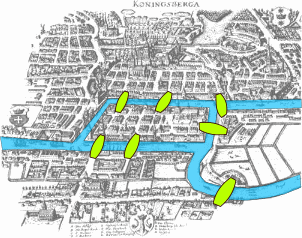
\includegraphics[width=0.3\linewidth]{chapter1/Konigsberg_bridges.png} \hspace{2cm}
	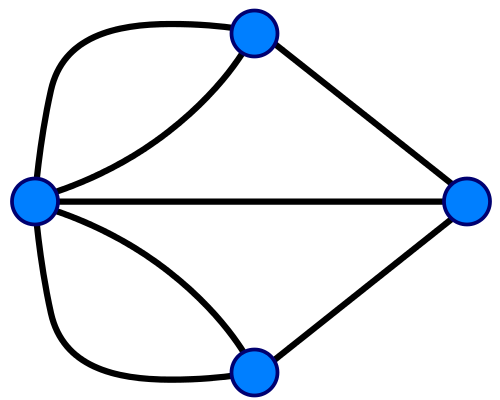
\includegraphics[width=0.3\linewidth]{chapter1/Konigsberg_graph.png}
	\caption[\selectlanguage{english}Konigsberg problem of seven bridges.]{The Kronigsber problem of seven bridges. The left panel shows the original map of the bridges; the right panel shows its graph representation. }
	
	\label{fig:Krgraph}
\end{figure}

Until the late 1990s, graph theory was not widely used. Back then, the most crucial model was the Erdos-Reni model of random graphs, which considers a fixed number of nodes in the network connected randomly, resulting in the Poisson degree distribution. When researchers got an idea to map the World Wide Web (WWW) on the network and analyse its properties \cite{huberman1999}, they found that degree distribution follows the power-law contrary to expected behaviour from random graph model \cite{dorogovtsev2010complex}. Because the power-law distribution is the same on all scales, such networks are called scale-free. Besides the scale-free property, empirical analysis of various complex networks showed the small-world property, and the high clustering coefficient \cite{barabasi2009,newman2010}. Two seminal papers from 1999 inspired further research in complex networks. Watts and Strogatz \cite{watts1998collective} proposed the model where rewiring of edges on regular lattice leads to the network in which paths between any two nodes become small (small-world) and nodes become densely connected, resulting in a high clustering coefficient. On the other hand, Barabasi and Albert (BA) \cite{barabasi1999} introduced the model, where the network grows over time, and the new nodes tend to connect high-degree nodes; it produces scale-free networks with few highly connected nodes. 

Different complex network models were proposed to describe the structure and dynamics of social and technological systems. The node degree is one of many node features that determine the linking probability, and the linking probability may be nonlinear in node degree or may depend on the age of the node \cite{dorogovtsev2000b, dorogovtsev2001b}. In the BA model, the links are introduced through new nodes, so it was proposed that links can be created between existing nodes in the network.  

Furthermore, the BA model considers the constant network growth, where a fixed number of nodes is added at each step. The research on various social systems shows time-dependent growth, and we record the exponential growth of online systems \cite{liu2019}. Some models considered that nodes become inactive or even that network grows through a nonlinear number of links \cite{pham2016}. On the other hand, models with accelerated growth in the number of nodes \cite{sen2004} simulate exponential expansion of the online social systems. But the growth is not only accelerated; the time series of new nodes has trends and reflect the typical human behaviour \cite{mitrovic2010a, mitrovic2012,mitrovic2015}.

Research has also been devoted to using generated networks to analyse dynamic processes on top of them. Central questions are about the spread of epidemics, information diffusion, or emotional interactions among elements \cite{garas2012emotional}. These systems are modelled using agent-based models, while the robustness is often studied by percolation and diffusion phenomena in complex networks. It was shown that scale-free networks' connectivity is sensitive to removing highly connected nodes. On the other hand, eliminating small degree nodes won't affect the scale-free structure \cite{cohen2000resilience}. They also show resilience to random attacks. Real-world networks are often characterised by community structure. They are common for social networks, where people with similar interests group together. Mostly adopted definition of a community is a group of densely connected nodes. The complex network theory provides different models for generating networks with community structure but also develops the algorithms for inferring the community structure from the underlying network. 

%Studies about the dynamics and structure of complex networks are necessary for understanding underlying mechanisms that shape complex systems. 
The complex network models contribute to our knowledge, connecting the network topology and the dynamics of the system and helping us to understand underlying mechanisms that lead to the emergence of the properties of the complex networks \cite{barabasi1999, tadic2001, mitrovic2009, ghoshal2013uncovering}. %Uncovering the role of elementary processes in network evolution \cite{ghoshal2013uncovering}. 
Complex network models must gain insights based on empirical data and social theories, and they are data-driven and require the development of computational approaches. The physicists showed interest in modelling complex systems by applying statistical physics approaches. Recently, the theory of graph neural networks (GNN) emerged from computer science, where machine learning methods are found helpful in inferring the properties of the network. For example, they are used to determine missing links and recommend to users in online social networks or to develop generative GNN models that lead to the discovery of new drugs.  

Real networks are much more heterogeneous than networks obtained in simple models. Links may be directed or undirected, they may have temporal dependencies, or we can deal with different types of interaction in one system. Other network representations deal with these specific features. In the following section, we will introduce complex networks and different approaches to deal with particular data types. 

\section{The complex networks}
%TODO Ovaj section mi je OK do na primere. Kao sto si na primer istakla da WWW primer usmerene mreze, ne bi bilo lose da za svaki tip mreze imamo neki primer i citat

The graph or network $G$ is defined as $G=(\boldsymbol{V}, \boldsymbol{E})$, where $\boldsymbol{V} = \{ v_1, v_2, ... v_N\}$ is a set of $N$ nodes (vertices), and  $\boldsymbol{E} = \{e_1, .. e_L\}$ is a set of $L$ edges (links). The edge is pair of nodes $e = (v_i, v_j), $ such that $\{v_i,v_j\}\in \boldsymbol{V}$. The most basic network representation considers \textbf{unweighted and undirected} structure. The edges are unweighted, meaning that all interactions in the network are equally important. Because the network is un-directed, edges are symmetric, so $(v_i, v_j)$ implies $(v_j, v_i)$. In \textbf{directed} networks, this symmetry is broken. The interaction between two nodes, $v_i$ and $v_j$, can be only in one direction. A typical example is World Wide Web, where webpages are nodes and hyperlinks are directed edges. In biological networks, gene regulation and neural activation can be described as a directed network. The first column a) in Figure \ref{fig:graph_dir} shows the graphical representation of two networks with an equal number of nodes; the first is undirected, and the second is directed. 

Even though graphical representation can be useful for describing the network structure, mathematical representation allows us to characterise the statistical properties of the networks. The graph $G$, with $N$ nodes could be represented with \textbf{adjacency matrix} $|A| = N \times N$ \cite{boccaletti2006complex}. The matrix elements are positive if there is a connection between two nodes $v_i$ and $v_j$. 
\begin{equation}
A_{ij} =
\begin{cases}
1 & \text{ ($v_i$, $v_j$) $\in$ $E$}\\
0 & \text{ ($v_i$, $v_j$) $\notin$ $E$}
\end{cases}       
\end{equation}

Column b) on Figure \ref{fig:graph_dir} shows the adjacency matrix representation of given graphs. By convention, as self-loops are not allowed, diagonal elements $A_{ii}=0$. For an undirected network adjacency matrix is symmetric $A_{i,j}=A_{ji}$, but in the case of a directed network matrix is not symmetric, as edges are drawn in one direction only.  

\begin{figure}[h]
	\centering
	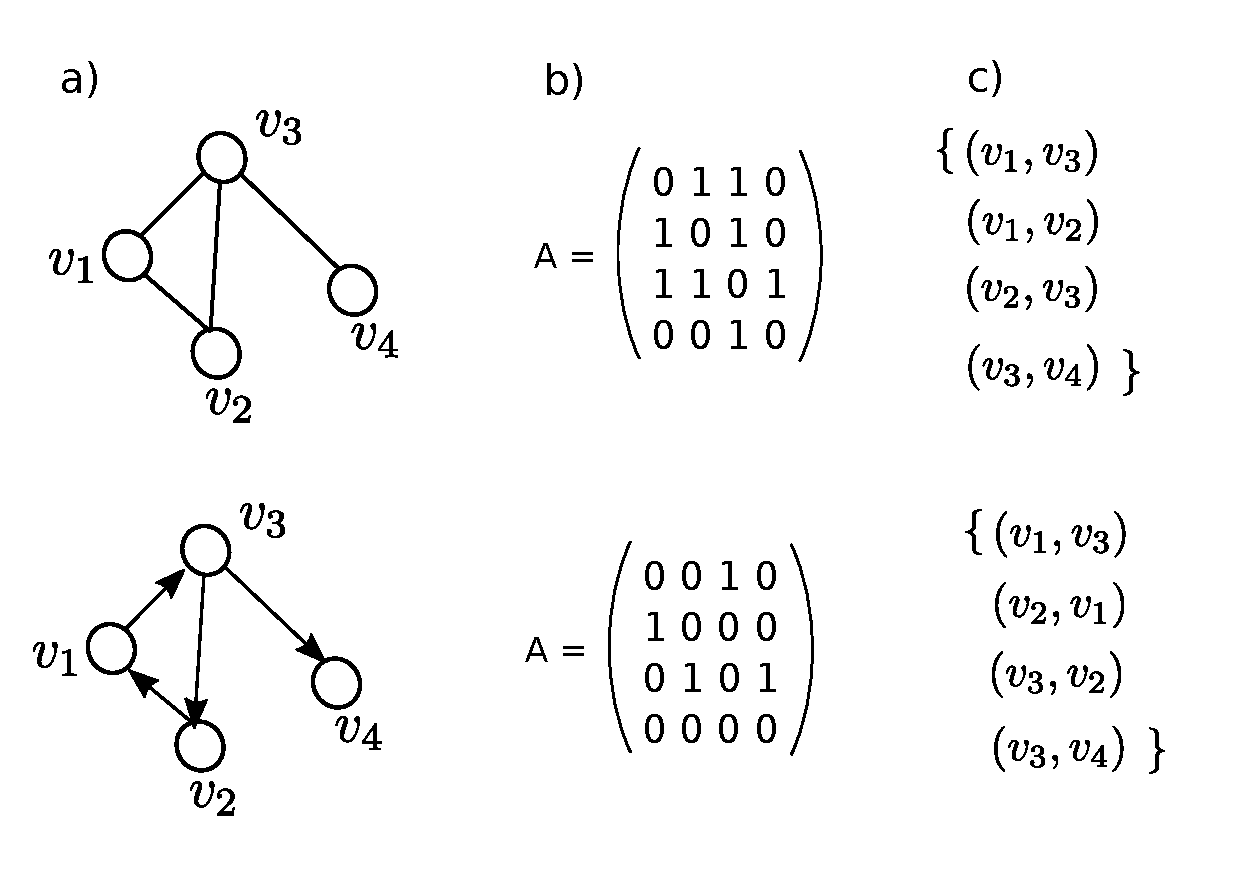
\includegraphics[width=0.7\linewidth]{chapter1/directed_graph.pdf} 
	\caption[Graph, matrix and edge list representations.]{a) Graph representation of undirected (top panel) and directed (bottom panel) network. The same networks are represented with adjacency matrices in column b) and edge list representation in column c).}
	\label{fig:graph_dir}
\end{figure}

The number of edges and nodes are dependent variables. Considering that each node can make $N-1$ connections, the maximum number of the edges in the network is $L_{max}=N(N-1)/2$, as each edge is counted twice. For a directed network, it is possible to draw $L_{max}=N(N-1)$ edges \cite{caldarelli2007scalefree}. When it comes to large networks, they are sparse, meaning that the number of links is $L<<L_{max}$. Consequently, the adjacency matrix is also a sparse structure (has many zeros) that takes a large portion of computer memory \cite{barabasi2016network}. 
It is common to represent the graph as an edge list. In this case, illustrated in Figure \ref{fig:graph_dir}, column c), a graph is described with the list of links that are in the graph, $G = \{ \{v_i,v_j\}\}$. Still, with this representation, we cannot distinguish between directed and undirected graph structures, so the computational algorithm should specify if the edges are symmetric or not.  


\begin{figure}[h]
	\centering
	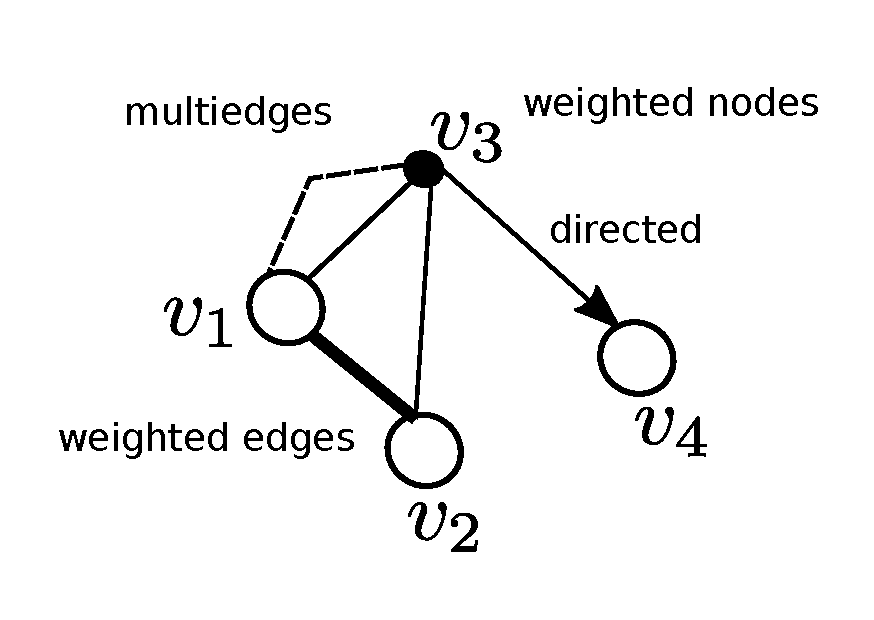
\includegraphics[width=0.4\linewidth]{chapter1/multi_graph.pdf} 
	\caption[Different network representations.]{The complex networks may represent different system characteristics. The edges can be directed, weighted or multiply. Also, nodes can be assigned with different weights or any relevant feature.}
	\label{fig:multigraph}
\end{figure}

Sometimes is essential to include the specific properties of the system in the network representation. For example, to emphasise the frequent interactions between nodes, edges can be assigned with different values; such networks are \textbf{weighted}. They can be described with an adjacency matrix, whose elements can take any real number $A_{ij}=w_{ij}$ and $w_{ij}>0$. In general, edges may be associated with any categorical variable. Similarly, properties can be added to nodes or the whole network structure. Edges could be characterised by the time when the interaction between nodes happens, which includes the \textbf{temporal} component in the network representation. Finally, if two nodes interact differently, the \textbf{multigraph} is an appropriate configuration where multiple edges are allowed. Figure \ref{fig:multigraph} presents the graphical representation of discussed network representations.

A \textbf{bipartite network} consists of two types of nodes. The nodes in the same partition are not connected, while links exist only between partitions. For many real systems, a bipartite graph is a natural representation\cite{barabasi2016network, latora2017complex}. For example, the bipartite network of people and groups has two distinct node partitions, while links indicate the memberships. Another example is a system of customers and products. The user and item link is created when the user buys an item. The bipartite networks find their application in the algorithms for recommended systems, whose goal is to suggest items that may interest the user. Actually, to find the most probable missing links in the network. 

In a bipartite network, nodes in one partition are not connected. Still, we can analyse a single node type if we project the bipartite network on one partition. The primary assumption is that two nodes in one partition could be connected if they point to the same node in another partition. Consider the network of movies and actors. The one-mode projection of movies is an undirected network whose links indicate that two movies share the same actors. On the other hand, another projection is a network of actors. The links exist if two actors appear in the same movie \cite{newman2010, barabasi2016network}.

\begin{figure}[h]
	\centering
	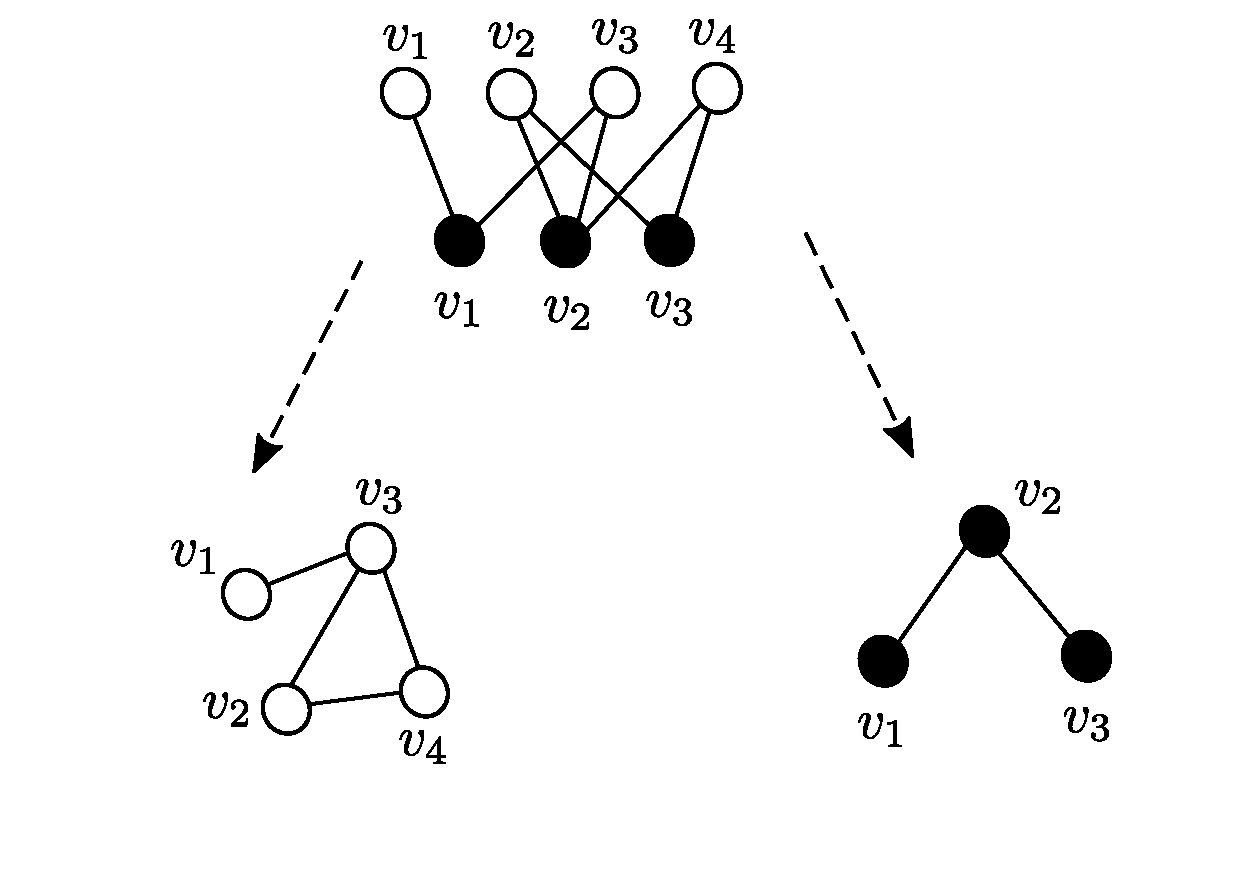
\includegraphics[width=0.7\linewidth]{chapter1/bipartite_graph.pdf} 
	\caption[Bipartite network.]{Bipartite network and two partition projections.}
	\label{fig:gt2}
\end{figure}

We should be aware that important information is lost when creating a one-mode projection. First, having weighted edges in the network of actors is necessary to know how many movies two actors appear. From the one-mode projection, we can not reconstruct the original network. Moreover, two different bipartite networks may have the same projected networks. The important consequence of the network projection is the creation of cliques, i.e. subgraphs where all nodes are connected. \\
In general, it is possible to define the k-bipartite network. The same rules apply as before. There are $k$ distinct node partitions, while the edges exist only between different types of nodes.

\textbf{Temporal networks.}
Studying real systems as static networks can give us a lot of insight into the system's properties. Still, real systems are not static; they evolve not only in the number of elements but also in the number of interactions between them. Some interactions in the system may repeat in different intervals and could be described with complex activity patterns. Including time dimension in the network, representation allows us to study the properties of the system closely. The temporal information may matter a lot \cite{holme2012}. For example, if the interaction between nodes $(v_1, v_2)$ happened before in time than  $(v_2, v_3)$, then nodes $v_1, v_3$ would not be connected, as is the case in the static network. 

The temporal network is a collection of timestamped edges. Each edge is defined as $(v_i, v_j, t, \Delta t)$, where $v_i$ and $v_j$, are nodes $t$ is time when interaction happen, and $\Delta t$ is event duration \cite{guide_temporal}. The duration of the events may vary, as in the phone-call network. Also, for many systems, the time resolution of the event duration is too small. For example, this parameter may be neglected when people interact on social platforms or email each other because the event time is too short; it scales in seconds.

\begin{figure}[h]
	\centering
	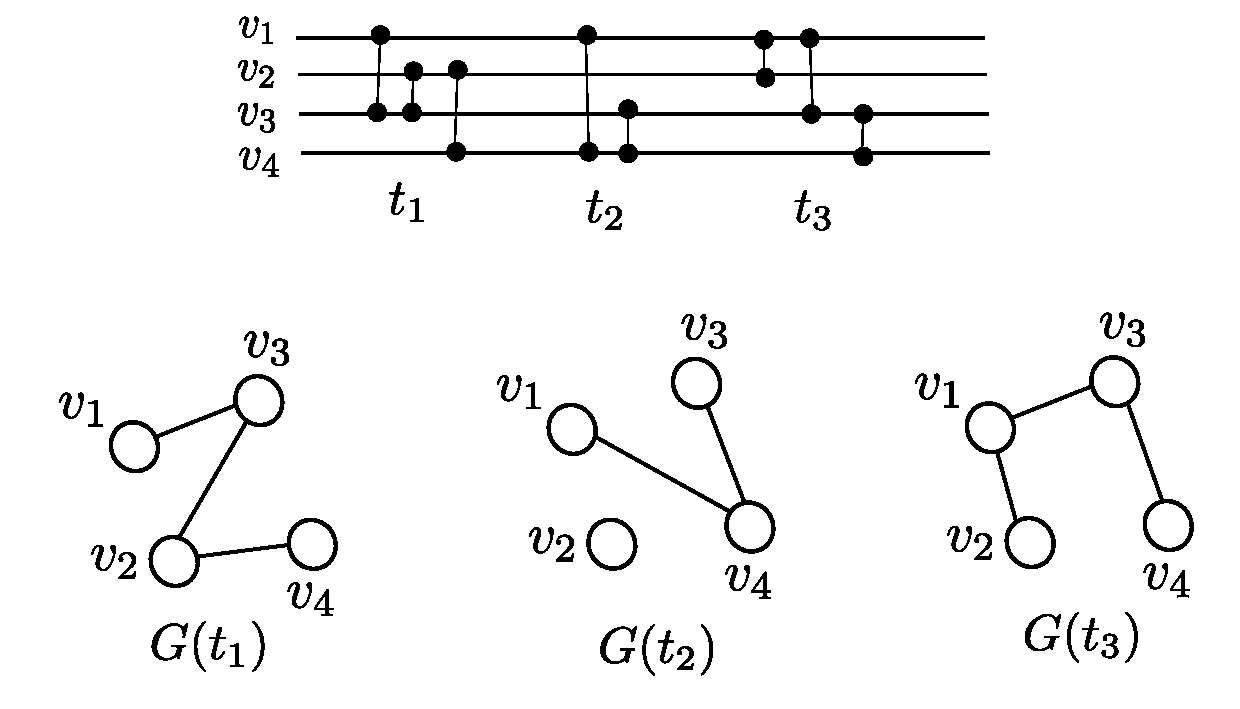
\includegraphics[width=0.7\linewidth]{chapter1/temporal_network.pdf} 
	\caption[Temporal network.]{Temporal network. }
	\label{fig:gt3}
\end{figure}

The temporal network can be represented as a sequence of static networks that evolve in time, $G = \{ G(t_1), G(t_2), ..., G(t_{max})\}$. At each time step, we can create the network and analyse the macroscopic properties of the given network snapshot. With this, we can end up with graph snapshots with many disconnected components or empty graphs for some points \cite{holme2015modern}. Sometimes, a much better approach is to aggregate the links that, over time windows. Here, we need to specify the time window length $w$. Interactions in the time interval $0\leq t<w$ enter the first snapshot. The following snapshot takes edges $w \leq t <2w$, and so on. The time windows are not overlapping, but generally, it is possible to slide the time window for different periods $ 1 \leq \delta t \geq w$. The downside of this method is that we can not recover original data points. The larger the time window is, the more information is lost. If the time window is set to $w=t_{max}$, there is only one snapshot, and the temporal data are no more available \cite{krings2012effects, arnold2021moving}. 

\textbf{Multilayer networks} were introduced for studying systems in which different types of interaction exist. This formalism allows one to investigate diverse network systems and to combine different types of data into one model \cite{porter2018multilayer}. In a multilayer or multiplex network, all nodes are present in each layer, but their interactions among layers differ. Two nodes may be connected in one layer but not in the other. Different online social systems may be an example of a multiplex network when users are connected on one platform but not on the other \cite{aleta2019multilayer}. Or the airline transportation network, where each layer represents the flights of different airline companies \cite{kivelamultilayer}.  


\section{In this thesis}
%TODO Ovde mi samo nedostaje jedan paragraf koji kaze koje probleme proucavamo, na kojim sistemima i kako se oni povezuju sa temom.

This thesis uses statistical physics and complex network approaches to model and empirically analyse online social systems. These systems consist of many users interacting online and could be represented by complex networks. In chapter \ref{Ch:Method}, we provide the methodology employed for this research. We describe the fundamental measures of complex networks and introduce basic complex network models. We review the most common probability distributions characterising complex systems' properties and outline distribution fitting methods. Finally, we introduce the multifractality of the time series and dynamical reputation model. 

Chapter \ref{Ch:signals} addresses the difference between network models where the growth in a number of nodes is constant and when it follows a non-trivial growth signal. This research aims to quantify how growth signals influence the structure of complex networks. Using the adapted ageing model \cite{hajra2004}, we use computer simulations to generate different kinds of complex networks. For more realistic real-world network simulations, growing signals are time series of new users from online social platforms, MySpace and Tech group from Meetup. They are described with trends, cycles and long-range correlations. Often time series have multi-fractal properties. The results of this study are published in \cite{vranic2021growth}, and they show the importance of growth signals in shaping the network structure because the scale-free networks, which represent real systems, are mainly altered. 

As research on social groups mainly focuses on a single group, there are remaining questions about the characteristics of the entire system. For example, the Tech group is only one of the groups around which Meetup users organise; many other groups are created worldwide, so the system constantly grows. In chapter \ref{Ch:Groups}, we will examine how groups on online social platforms grow. The results are summarised in the paper  \cite{vranic2022universal}. This research is based on Reddit and Meetup data. From Meetup, we created two data sets, one with groups created in London and the other with groups created in New York, while for Reddit, we selected groups built before 2012. We are interested in explaining scaling behaviour in group size and growth rate distributions and identifying the growth mechanisms present in the system. Using a bipartite complex network model, we can reproduce the universality found in the system.

Even though across complex systems, we find the emergence of universal behaviour, for example, the scaling of the degree distribution of two groups is similar, different factors might influence its success. It is well known that many online groups may suddenly fall apart. These questions are the subject of the chapter \ref{Ch:Trust}, which main results are published in the paper \cite{vranic2022sustainability}. Here, we study the question-answer platform Stack Exchange; it has more than 200 different topic-specified sites where people help each other answer questions. What is interesting about this system is that some sites were closed because they did not produce enough activity. For that reason, we selected the sites with the same topic that failed but later, when someone proposed the site again, it stayed active. We analyse the evolution of user interaction networks; here, we use the temporal network approach and compare active and closed sites. We find that it is essential how the network users are distributed into a core-periphery structure \cite{gallagher2020clarified}. The core must select firmly connected users, but their interaction with the periphery has to be high. In other words, we need a trustworthy core to hold the community. Introducing the Dynamical Reputation Model (DIBRM) \cite{melnikov2018toward}, based on user interaction sequences, we quantify how much users can be trusted and whether the community has a strong core. In the appendix \ref{App:SE}, we briefly describe the Stack Exchange sites. In appendix \ref{App:parameters} and \ref{App:sliding} discuss how we choose parameters for the DIBRM model, while in appendix \ref{App:robust} we discuss the stability of inferred core-periphery structures. 

Finally, in chapter \ref{Ch:Conclussion}, we draw the main findings of this thesis. 


\selectlanguage{english}














